\documentclass[11pt,a4paper]{article}
\usepackage[utf8]{inputenc}
\usepackage[margin=1in]{geometry}
\usepackage{amsmath,amssymb}
\usepackage{booktabs}
\usepackage{hyperref}
\usepackage{microtype}
\usepackage{enumitem}
\usepackage{tikz}
\usepackage{placeins}
\usetikzlibrary{shapes.geometric, arrows, positioning}
\setlength{\emergencystretch}{3em}

\hypersetup{
    colorlinks=true,
    linkcolor=blue,
    filecolor=magenta,
    urlcolor=blue,
    pdftitle={Literature Review: Toward Signal-Preserving TinyML for Gravitational Wave Triggers},
    pdfpagemode=FullScreen,
}

\title{\textbf{Literature Review: Toward Signal-Preserving TinyML for Gravitational Wave Triggers} \\
\large Resolving the Tension Between Astrophysical Fidelity and Sub-Watt Model Compression}
\author{\textbf{Razeen Wasif} \\ Uni ID: u7283652 \\ Course Code: COMP4450}
\date{May 25, 2026}

\begin{document}

\maketitle

\begin{abstract}
Detection of compact-binary coalescences within the millisecond budget of multi-messenger astronomy is now constrained by hardware as much as by algorithms. This review synthesises eighteen papers from gravitational-wave (GW) machine learning, embedded inference, and quantisation theory to ask whether the trigger stage of a GW pipeline can be pushed onto sub-watt microcontrollers without losing astrophysical sensitivity. The literature separates into two weakly connected camps. One has shown that deep networks can match matched filtering on high-power GPUs. The other has shown that aggressive compression is feasible, but evaluates it on images and audio rather than on chirp waveforms. The hinge between the two is low-bit integer quantisation, which acts on a phase-coherent waveform as a structured perturbation rather than the well-behaved rounding error assumed by computer-vision benchmarks. Existing quantisation-aware training and distillation work does not address this, leaving a clear opening for physics-informed, signal-preserving compression.
\end{abstract}

\noindent\textbf{Keywords:} TinyML; quantisation-aware training; gravitational-wave detection; signal-to-noise ratio; embedded machine learning; low-latency triggers; multi-messenger astronomy.

\smallskip
\noindent\textbf{ACM CCS:} Computing methodologies $\rightarrow$ Machine learning algorithms; Computer systems organization $\rightarrow$ Embedded systems; Applied computing $\rightarrow$ Astronomy.

\section{Introduction}

\subsection{Summary of the Research Proposal}
This review provides the literature foundation for the COMP4450 Research Proposal \textit{``Quantisation-Induced SNR Degradation: Toward Signal-Preserving TinyML for Gravitational Wave Triggers''} (Wasif 2026). The proposal sits at the intersection of \textit{Intelligent Systems} (primary), \textit{Embedded Computer Systems}, and \textit{Computational Astrophysics} (secondary). Its central claim is that next-generation gravitational-wave detectors face a data-deluge problem GPU-bound deep-learning pipelines cannot solve. Missions such as LISA and CubeSat-scale autonomous arrays cannot downlink raw data, so the trigger stage must move onto sub-watt microcontrollers with approximately 256~KB of SRAM. That move forces aggressive low-bit integer quantisation, and the proposal asks how bit-width reduction interferes with the phase coherence on which reliable GW triggering depends.

\subsection{Aim and research questions}
The aim of this review is to survey the literature that approaches the gap from two directions: GW machine learning on one side, and TinyML and quantisation theory on the other. The case made here is that the intersection remains unresolved. Two questions structure the survey. \textit{RQ1} asks how prior work has traded model size, latency, and astrophysical sensitivity. \textit{RQ2} asks which quantisation-aware techniques, if any, have been validated against astrophysical metrics such as false alarm rate and distance reach, rather than against the top-1-accuracy metrics inherited from computer vision. The technical context matters here. Detecting dimensionless strains of $h \approx 10^{-21}$ by matched filtering is statistically optimal but computationally heavy (Abbott et al.\ 2020), and template-bank growth is now the limiting factor in multi-messenger follow-up (Cuoco et al.\ 2024). Deep learning matches matched-filter sensitivity in published results (George and Huerta 2018; Gabbard et al.\ 2018), but those results all assume FP32 arithmetic. What happens when that arithmetic is compressed to INT8 is the question this review traces.

\section{Materials and Methods}

A targeted, reproducible review was conducted between March and April 2026. It is lighter than a formal systematic review, but disciplined enough that someone else could re-run the search.

\subsection{Search strategy}
Four databases were used: arXiv (gr-qc, cs.LG, eess.SP), IEEE Xplore, the ACM Digital Library, and Google Scholar. Query strings paired GW terms (\textit{``gravitational wave'' OR ``binary black hole'' OR ``binary neutron star''}) with ML/hardware terms (\textit{``deep learning'' OR ``convolutional'' OR ``quantisation'' OR ``FPGA'' OR ``microcontroller'' OR ``TinyML''}). GWOSC was checked for datasets and observational papers, and citation chasing used George and Huerta (2018), Gebhard et al.\ (2019), and Gholami et al.\ (2021) as seeds.

\subsection{Inclusion and exclusion criteria}
Papers were included if they did one of three things: propose or evaluate a machine-learning model for GW detection, denoising, or triggering; supply foundational work on quantisation, distillation, or embedded inference; or report quantitative sensitivity or efficiency results. Papers were excluded if they focused only on offline Bayesian parameter estimation, cosmology without a trigger stage, or post-hoc visualisation. Murphy et al.\ (2021) is included as an autonomous, downlink-constrained deployment analogue. Messick et al.\ (2017) supports the hierarchical-trigger argument in §3.6, but is not one of the 18 in-depth synthesis targets.

\subsection{Inclusion outcome}
Eighty-six records were identified. After deduplication and title/abstract screening 32 remained for full-text assessment, and 18 were finally included for in-depth review (Figure \ref{fig:prisma}). The included set divides into four thematic groups: seven papers showing ML matching matched filtering, four on quantisation theory and embedded frameworks, three on FPGA-class hardware deployment in physics, and four critical or foundational papers on noise, glitches, and benchmarks. A second, orthogonal axis (contribution type) is used in §3 to map the same 18 papers onto sensitivity, efficiency, and robustness. Papers are double-counted where they bridge cliques — Chaturvedi et al.\ (2022), for example, spans sensitivity-first and hardware co-design — so the two axes do not produce the same counts, and the §3 subsection totals sum to more than 18.

\subsection{Validity}
Three measures support reproducibility. First, every included paper is cited with a DOI or arXiv ID, so the search can be replicated in five years. Second, a ``clique map'' was maintained that assigns each paper to one or more of three thematic axes (sensitivity, efficiency, robustness). The map makes visible where the literature is thick and where it is thin. Third, claims were cross-checked between independent works. The adversarial-noise critique of George and Huerta (2018) by Gebhard et al.\ (2019) is one example, and Banbury et al.'s (2021) microcontroller benchmarks, when read against the SRAM budgets assumed by David et al.\ (2021), are another.

\begin{figure}[htbp]
\centering
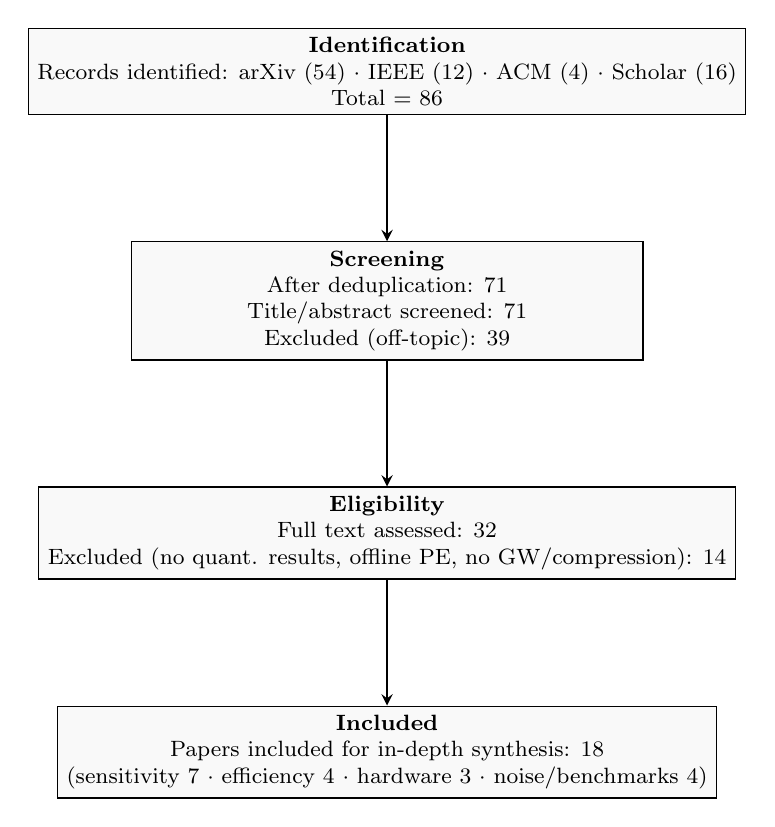
\begin{tikzpicture}[
  node distance=1.6cm,
  box/.style={draw, rectangle, minimum width=6.5cm, minimum height=1cm, align=center, fill=gray!5, font=\footnotesize},
  arrow/.style={thick,->,>=stealth}
]
  \node (ident) [box] {\textbf{Identification} \\ Records identified: arXiv (54) $\cdot$ IEEE (12) $\cdot$ ACM (4) $\cdot$ Scholar (16) \\ Total = 86};
  \node (screen) [box, below=of ident] {\textbf{Screening} \\ After deduplication: 71 \\ Title/abstract screened: 71 \\ Excluded (off-topic): 39};
  \node (elig) [box, below=of screen] {\textbf{Eligibility} \\ Full text assessed: 32 \\ Excluded (no quant. results, offline PE, no GW/compression): 14};
  \node (incl) [box, below=of elig] {\textbf{Included} \\ Papers included for in-depth synthesis: 18 \\ (sensitivity 7 $\cdot$ efficiency 4 $\cdot$ hardware 3 $\cdot$ noise/benchmarks 4)};

  \draw [arrow] (ident) -- (screen);
  \draw [arrow] (screen) -- (elig);
  \draw [arrow] (elig) -- (incl);
\end{tikzpicture}
\caption{PRISMA-style flow of identification, screening, eligibility, and inclusion.}
\label{fig:prisma}
\end{figure}

\section{Results}

\noindent\textbf{Key message.} The literature splits into two weakly connected cliques. A sensitivity-first clique (George and Huerta 2018; Gabbard et al.\ 2018; Krastev 2020; Schäfer et al.\ 2023; Dax et al.\ 2021; Chaturvedi et al.\ 2022) shows that deep learning can match matched filtering, but only on GPU. A deployment-first clique (David et al.\ 2021; Banbury et al.\ 2021; Gholami et al.\ 2021; Jacob et al.\ 2018; Hinton et al.\ 2015) shows that aggressive compression is feasible, but evaluates models on generic benchmarks rather than astrophysical strain. Critical papers (Gebhard et al.\ 2019; Abbott et al.\ 2016; Abbott et al.\ 2020) warn that these models are fragile in ways simple accuracy metrics cannot detect. On a separate contribution-type axis, the included papers map roughly to sensitivity, efficiency, and robustness, but no paper contributes primarily on all three. Figure \ref{fig:bitwidth} projects the same literature onto the axes the proposal's hypothesis actually lives on: weight precision and sensitivity preservation.

\subsection{The sensitivity-first clique}
George and Huerta (2018) and Gabbard et al.\ (2018) form the foundation of ML-based GW detection. Both show that a relatively shallow one-dimensional CNN can recover binary black hole (BBH) signals from Advanced LIGO strain at sensitivity comparable to matched filtering. They are best read as a clique: they converge on the same architectural choice (deep 1-D convolutions over whitened strain) and report the same null result (no measurable loss of true-positive rate at high SNR), so their joint claim is stronger than either paper alone.

Krastev (2020) extended the design to binary neutron star (BNS) signals, and in doing so surfaced a constraint the BBH papers had not encountered. BNS waveforms are an order of magnitude longer in the detector band, so the receptive field of any TinyML candidate model has to grow proportionally. That requirement runs directly into the SRAM budget assumed by David et al.\ (2021).

Schäfer et al.\ (2023) formalised the comparison through the first ML mock-data challenge. The headline result was that ML pipelines were competitive with PyCBC at high false-alarm-rate thresholds, but lagged at the low-FAR regime that astrophysical confirmation actually requires. Dax et al.\ (2021) and Chaturvedi et al.\ (2022) close out the clique on the inference side. The former demonstrates real-time \textit{posterior} estimation in seconds. The latter applies NVIDIA TensorRT FP16 mixed-precision and graph-optimisation layer fusion, reporting processing of one month of Advanced LIGO data (both Hanford and Livingston streams, August 2017) in approximately 50 seconds, a roughly $3\times$ speedup over the unoptimised AI baseline, with no measurable sensitivity loss for known BBH events. The limitation is that this result depends on A100-class datacentre GPUs and TensorRT calibration, not on memory-static microcontroller inference. The collective blind spot of the clique is therefore hardware scale.

\subsection{The deployment-first clique}
Where the sensitivity clique assumes GPUs, the deployment clique assumes microcontrollers. David et al.\ (2021) define the de facto runtime for TinyML in the form of TensorFlow Lite Micro, and lay out the engineering primitives that govern what can and cannot run in approximately 256~KB of SRAM: a single pre-allocated tensor arena, op-by-op execution, no dynamic allocation after initialisation, and vendor-specific kernels such as CMSIS-NN. Their evaluation reports interpreter overhead below 0.1\% for large models. Banbury et al.\ (2021) supply the calibrating benchmark suite (MLPerf Tiny), which covers keyword spotting, visual wake words, image classification, and anomaly detection, not astrophysical time series.

The theoretical machinery sits with Gholami et al.\ (2021), whose taxonomy of post-training quantisation (PTQ) and quantisation-aware training (QAT) is the canonical reference, and with Jacob et al.\ (2018), whose integer-arithmetic-only inference paper supplies the mathematical foundation, applying the straight-through estimator to propagate gradients through the rounding operator during training. Knowledge distillation (Hinton et al.\ 2015) is the complementary tool: a high-precision teacher transfers softened class probabilities to a quantised student, recovering accuracy PTQ discards.

The clique is internally coherent and well-cited. But its evaluation regime is uniformly computer-vision-centric: top-1 ImageNet accuracy, word-error rate, mean average precision. None of these metrics quantifies the loss of phase coherence that matters for a chirp signal. That gap is the central observation of this review.

\subsection{Quantisation as algorithmic detector noise}
Gebhard et al.\ (2019) is the critical pivot of the review. It re-examines the George and Huerta (2018) and Gabbard et al.\ (2018) results, and shows the high reported accuracies disguise something the authors did not test for: adversarial brittleness. Small, structured perturbations to the input strain flip the network output with high confidence, and the network confidently classifies inputs that bear no visible resemblance to a chirp. Gebhard et al.\ conclude that CNNs should be used as trigger generators only, not as confirmation tools.

Abbott et al.\ (2016) catalogue the morphology of ``blip'' transients in real LIGO data. These are exactly the kind of high-amplitude, short-duration response a quantised CNN is most likely to misclassify. Abbott et al.\ (2020) document the data-quality vetoes the LVK collaboration uses to mitigate them offline.

Three structurally distinct sources of detector noise therefore threaten an ML-based GW trigger: instrumental glitches in the strain itself (Abbott et al.\ 2016; Abbott et al.\ 2020); adversarial perturbations of the learned decision surface (Gebhard et al.\ 2019); and the algorithmic noise injected by the inference pipeline, of which low-bit integer quantisation is the largest single contributor (Gholami et al.\ 2021; Jacob et al.\ 2018). Treating quantisation as a third source of detector noise, algorithmic rather than instrumental, is the conceptual move this review proposes. It also explains why computer-vision quantisation results do not transfer to GW triggers: image and audio benchmarks have no analogue of detector noise, so quantisation error there is well modelled as bounded rounding under the standard quantisation noise model (Gholami et al.\ 2021), whereas in a GW trigger it is a structured perturbation that interacts with chirp phase evolution and therefore directly affects astrophysical sensitivity. None of the deployment-first papers acknowledge this, which is a serious omission.

\subsection{Hardware-software co-design on FPGA-class targets}
A small group of papers sits between the two cliques and provides the closest evidence for the proposal's hardware claim. Martins et al.\ (2025) implemented a \texttt{WaveNet}-based CNN for BNS early warning on an FPGA, using \textit{power-of-two (logarithmic) quantisation} via Vitis AI rather than uniform INT8. Their headline result improves detection accuracy at 1\% false-alarm probability from 66.81\% to 76.22\% over the prior leading ML-based early-warning system. On the FPGA, they report $\approx 84.5$~ms single-sample inference for FindCNN2D variants, and quantisation-induced accuracy changes from negligible (69.50\% $\to$ 69.37\%) through a 2~pp drop (79.42\% $\to$ 77.28\%) to a small improvement (71.72\% $\to$ 72.42\%). This is the clearest evidence that deployment precision can affect BNS trigger performance, but the metric is classification accuracy rather than SNR loss or distance reach, and the scheme is logarithmic rather than uniform INT8. Chaturvedi et al.\ (2022) span both cliques: their TensorRT result is on GPU, but it operationalises the same mixed-precision idea microcontroller deployments will need. Neither paper tests a sub-watt microcontroller, reports peak SRAM under a TinyML memory arena, uses astrophysical reach as a metric, or generalises the framework. The FPGA-class subset is therefore thinner than the §2.3 thematic count suggests — Martins is the only sub-watt-relevant hardware deployment in the included set, with Chaturvedi providing methodological adjacency on GPU. That thinness is itself part of the gap argument.

\subsection{Toward signal-preserving TinyML}
Cuoco et al.\ (2021) provide the earlier of two field-shaping reviews of ML in GW science; Cuoco et al.\ (2024) extend that coverage to current detectors. Neither devotes more than a paragraph to sub-watt deployment. The methodological building blocks for closing the gap already exist. Hinton et al.'s (2015) distillation framework supplies the training objective. Jacob et al.'s (2018) integer-only inference and Gholami et al.'s (2021) QAT taxonomy supply the quantisation machinery. What the literature does not contain is a composition of those blocks under astrophysical, rather than computer-vision, loss functions. Murphy et al.'s (2021) work on the EIRSAT-1 CubeSat gamma-ray detector illustrates the deployment niche the proposal is aimed at: a compact, autonomous, downlink-constrained instrument where on-board triggering is operationally required.

\subsection{The wrong benchmark}
The sensitivity-first clique evaluates ML detectors by matched-filter parity at fixed FAR. That benchmark suits confirmation, but an \textit{edge trigger} — a cheap first-stage classifier running on the detector side at sub-watt power — only needs to flag candidate windows cheaply enough for a higher-precision second stage. This hierarchy already exists: GstLAL is a rapid trigger feeding deeper analyses (Messick et al.\ 2017). Matched-filter parity at the trigger stage is therefore over-specification, and the FP32 assumption that helps meet it blocks TinyML deployment. Read this way, Martins et al.'s (2025) quantised-FPGA BNS result is not yet a microcontroller solution, but it suggests that small accuracy deltas may be acceptable if candidate recall and downstream load stay tractable. ``Signal-preserving'' therefore means preserving enough phase information for confirmation, not replacing matched filtering.

\begin{figure}[!htbp]
\centering
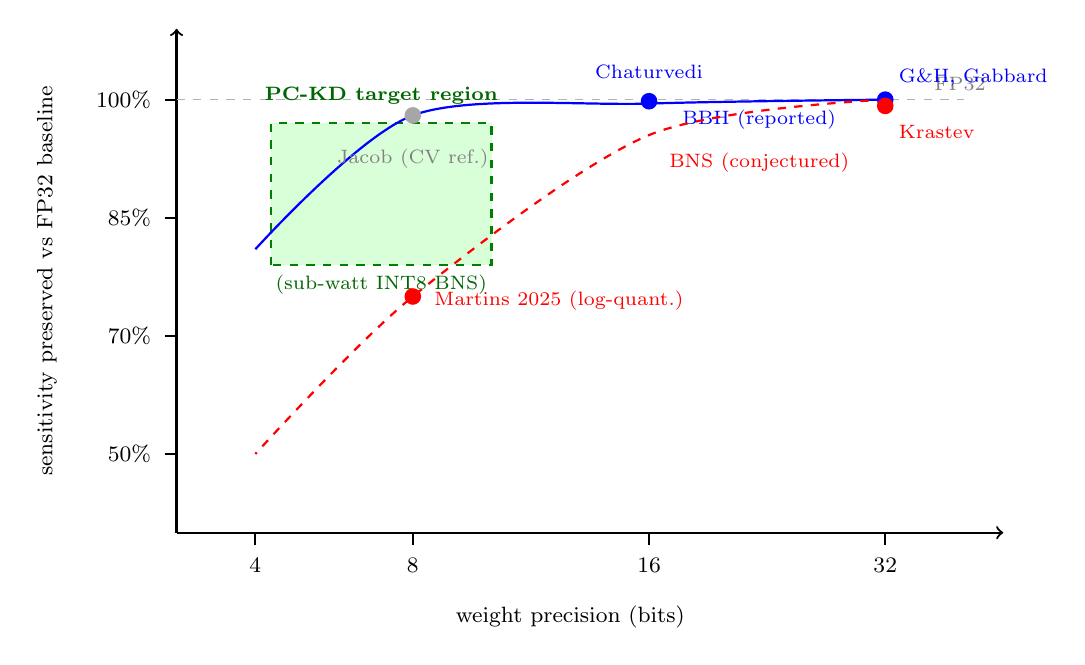
\begin{tikzpicture}[font=\footnotesize]

  % --- axes ---
  \draw[->, thick] (0,0) -- (10.5,0);
  \draw[->, thick] (0,0) -- (0,6.4);

  % x-axis ticks (log-spaced bitwidths)
  \foreach \x/\bits in {1/4, 3/8, 6/16, 9/32} {
    \draw[thick] (\x,0) -- (\x,-0.15);
    \node[below] at (\x,-0.2) {\bits};
  }
  \node[below, align=center] at (5,-0.8) {weight precision (bits)};

  % y-axis ticks (sensitivity preserved vs FP32 baseline)
  \foreach \y/\pct in {1.0/50, 2.5/70, 4.0/85, 5.5/100} {
    \draw[thick] (-0.15,\y) -- (0,\y);
    \node[left] at (-0.2,\y) {\pct\%};
  }
  \node[rotate=90, anchor=south] at (-1.4,3.2) {sensitivity preserved vs FP32 baseline};

  % FP32 baseline line
  \draw[dashed, gray!60] (0,5.5) -- (10,5.5);
  \node[gray, right, font=\scriptsize] at (9.5,5.7) {FP32};

  % --- target region (PC-KD aim, adjacent to Martins anchor) ---
  \fill[green!15] (1.2,3.4) rectangle (4.0,5.2);
  \draw[green!50!black, thick, dashed] (1.2,3.4) rectangle (4.0,5.2);
  \node[green!40!black, font=\scriptsize\bfseries, align=center] at (2.6,5.55) {PC-KD target region};
  \node[green!40!black, font=\scriptsize, align=center] at (2.6,3.15) {(sub-watt INT8 BNS)};

  % --- BBH curve (solid blue) ---
  \draw[blue, thick] plot[smooth, tension=0.5] coordinates {(9,5.5) (6,5.45) (3,5.30) (1,3.6)};
  \node[blue, font=\scriptsize] at (7.4,5.25) {BBH (reported)};

  % --- BNS curve (dashed red, hypothesised) ---
  \draw[red, thick, dashed] plot[smooth, tension=0.5] coordinates {(9,5.5) (6,5.05) (3,3.0) (1,1.0)};
  \node[red, font=\scriptsize] at (7.4,4.7) {BNS (conjectured)};

  % --- paper anchor points ---
  % BBH at FP32: George & Huerta 2018, Gabbard 2018
  \fill[blue] (9,5.5) circle (3pt);
  \node[blue, above right, font=\scriptsize] at (9.05,5.55) {G\&H, Gabbard};

  % BNS at FP32: Krastev
  \fill[red] (9,5.42) circle (3pt);
  \node[red, below right, font=\scriptsize] at (9.05,5.30) {Krastev};

  % Chaturvedi 2022: FP16 mixed-precision BBH (16-bit weights via FP16)
  \fill[blue] (6,5.48) circle (3pt);
  \node[blue, above, font=\scriptsize] at (6,5.65) {Chaturvedi};

  % Martins 2025: power-of-two quantised BNS on FPGA; accuracy delta, not reach
  \fill[red] (3,3.0) circle (3pt);
  \node[red, right, font=\scriptsize] at (3.15,2.95) {Martins 2025 (log-quant.)};

  % Jacob 2018: INT8 ImageNet (cross-domain reference)
  \fill[gray!70] (3,5.30) circle (3pt);
  \node[gray, below, font=\scriptsize] at (3,5.0) {Jacob (CV ref.)};

\end{tikzpicture}
\caption{Synthesis sketch of sensitivity preservation versus weight precision. BBH results remain close to FP32 through FP16 mixed precision (Chaturvedi et al.\ 2022), while BNS sensitivity is conjectured to degrade more sharply; Martins et al.\ (2025) provides the only GW low-bit deployment anchor in the included set, but uses power-of-two (logarithmic) quantisation rather than uniform INT8 and reports classification accuracy rather than SNR or distance reach. The green region is the \textit{target} PC-KD aims at — BNS-class sensitivity at INT8 or below on a sub-watt microcontroller — and is drawn adjacent to the Martins anchor rather than interpolated from it.}
\label{fig:bitwidth}
\end{figure}

\noindent The green target region in Figure \ref{fig:bitwidth} is the research gap PC-KD (\S4.3) is designed to fill. The slope of the BNS curve is hypothesised under the proposal's phase-coherence argument, not fitted from data; the figure encodes an argument, not a measurement.

\FloatBarrier

\section{Discussion}

\noindent\textbf{Key message.} The literature contains every ingredient required for signal-preserving TinyML, but no published work composes those ingredients under astrophysical loss functions. The single FPGA-class BNS deployment in the included set (Martins et al.\ 2025) evaluates quantised classification accuracy and hardware cost, but not SNR loss or distance reach. The gap is therefore one of evaluation discipline as much as of technique.

\subsection{Principal results}
Four findings emerge. First, deep learning reaches matched-filter parity for high-SNR BBH signals, but weakens at low FAR and on long-duration BNS waveforms (George and Huerta 2018; Gabbard et al.\ 2018; Schäfer et al.\ 2023). Second, embedded-ML measures quantisation cost in classification accuracy, not phase-coherent SNR loss (Jacob et al.\ 2018; Gholami et al.\ 2021; Banbury et al.\ 2021). Third, the only FPGA-class BNS deployment measures quantised accuracy and hardware cost under a power-of-two quantisation scheme, not astrophysical reach under uniform INT8 (Martins et al.\ 2025). Fourth, matched-filter parity is the wrong target for a first-stage edge trigger; under a hierarchical benchmark, Martins et al.\ (2025) is a partial success.

\subsection{Limitations}
Three limitations should be flagged. The 18-paper cap excluded adjacent work on mixed-precision FPGA inference outside astronomy and transformer-based GW pipelines. Some recent papers are arXiv preprints, so peer-review status varies. Figure \ref{fig:bitwidth} is also a coarse two-axis projection: it suppresses activation precision, layer-wise mixed precision, calibration choices, the distinction between uniform and logarithmic quantisation, and heterogeneity within BBH and BNS tasks. The BNS curve is hypothesised from one empirical anchor (Martins et al.\ 2025, under power-of-two quantisation) and should be redrawn as more uniform-INT8 BNS deployments appear. Finally, the PRISMA-style flow was conducted by a single reviewer rather than a panel, so selection bias is not formally controlled.

\subsection{Proposed future work: Phase-Coherence-Weighted Knowledge Distillation}
The target region of Figure \ref{fig:bitwidth} motivates a named contribution: \textit{Phase-Coherence-Weighted Knowledge Distillation} (PC-KD). PC-KD weights the student loss sample-by-sample by the time-frequency phase coherence of the input window against a chirp template. Quantisation noise in low-coherence regions is penalised softly; noise in late-inspiral and merger-adjacent regions, where phase evolution dominates SNR, is penalised hard. Concretely,
\begin{equation}
\mathcal{L}_{\text{PC-KD}}(x) \;=\; \alpha \, \tau^2 \, \mathrm{KL}\!\big( p_T^{(\tau)}(x) \,\|\, p_S^{(\tau)}(x) \big) \;+\; \beta \, w(x) \, \big\| f_T(x) - f_S(x) \big\|^2,
\label{eq:pckd}
\end{equation}
where $p_T^{(\tau)}, p_S^{(\tau)}$ are teacher and student class probabilities softened at temperature $\tau$ (Hinton et al.\ 2015), $f_T, f_S$ are penultimate-layer feature maps, and $w(x) \in [0,1]$ is a phase-coherence weight obtained by normalising the peak SNR of $x$ against a coarse, downsampled chirp template bank. The weight $w(x)$ is computed \textit{at training time only}, so the matched-filter pre-pass does not enter the microcontroller inference budget — the deployed student sees only its quantised forward pass. The KL term transfers teacher decisions; the weighted feature term is the astrophysical component, making compression care where quantisation error damages SNR. The asymmetric weighting — $w(x)$ on the feature term but not on the KL term — reflects that phase information is collapsed by the time it reaches the class-probability head but survives in penultimate-layer features; weighting where phase loss is observable is therefore the right place to weight. The matched-filter pre-pass that produces $w(x)$ runs once over the training set against a coarse template bank (approximately 100 templates is typically sufficient to discriminate inspiral-dominated from off-chirp windows), and $w(x)$ is cached per sample. $\alpha$ and $\beta$ are chosen by validation against FAR-controlled candidate recall on held-out injections, rather than against classification accuracy. PC-KD should be tested through microcontroller-class mixed precision (Chaturvedi et al.\ 2022), glitch diagnostics (Gebhard et al.\ 2019; Abbott et al.\ 2016; Abbott et al.\ 2020), and an MLPerf-Tiny-style benchmark parameterised by astrophysical reach (Banbury et al.\ 2021).

\subsection{Comparison with prior work}
Cuoco et al.\ (2021; 2024) review ML in GW science but treat hardware deployment as downstream engineering. Warden and Situnayake (2019), Lin et al.\ (2020), and Sze et al.\ (2017) survey embedded inference without astrophysical content. This review differs by treating the intersection as the problem, using Gebhard et al.\ (2019) and Martins et al.\ (2025) as load-bearing evidence, reframing matched-filter parity as the wrong trigger benchmark, and proposing PC-KD as a named methodological contribution.

\subsection{Conclusions}
TinyML for gravitational-wave detection cannot be achieved by stacking generic compression onto GPU-oriented ML pipelines. It also cannot treat quantisation as ordinary rounding or demand matched-filter parity from a first-stage trigger. The ingredients already exist: sensitive architectures, 256~KB-class runtimes, quantisation procedures, and distillation. What is missing is their composition under astrophysical metrics. PC-KD, as proposed in \S4.3, is the missing piece this review identifies; the Research Proposal that this review supports will operationalise it.

\section{Self-Reflection}
Generative AI was used in two roles: Google Gemini CLI for early section skeletons and reference discovery, and Anthropic Claude for one near-final cross-check. Every paragraph was rewritten by hand, and every AI-suggested reference was verified against the primary source before inclusion. The verification step did real work: an initial reference-discovery prompt returned plausible but unverifiable DOIs, which were caught during cross-checking and discarded; a refined prompt asking specifically for verifiable FPGA/CNN/BNS papers returned a smaller but reliable set, with Martins et al.\ (2025) the most useful hit. The main benefit of AI assistance was speed in moving between gravitational-wave physics and embedded systems vocabularies. The main risk was academic-integrity failure through fabricated or over-stated sources, mitigated by the verify-before-cite policy described above. For future work, summaries will be drafted from PDFs first, with generative AI used only for comparison or copy-editing on already-verified material.

\section*{List of References}

\noindent\textit{Entries marked with an asterisk (*) form the in-depth included set ($n = 18$). Unmarked entries below the divider are cited in support but were not subject to in-depth synthesis.}

\begin{enumerate}[label=\arabic*., leftmargin=2em]
\item Abbott, BP et al.\ 2016, `Characterization of transient noise in Advanced LIGO relevant to gravitational-wave signal GW150914', \textit{Classical and Quantum Gravity}, vol.\ 33, no.\ 13, 134001, doi:10.1088/0264-9381/33/13/134001. \url{https://doi.org/10.1088/0264-9381/33/13/134001}.*
\item Abbott, BP et al.\ 2020, `A guide to LIGO--Virgo detector noise and extraction of transient gravitational-wave signals', \textit{Classical and Quantum Gravity}, vol.\ 37, no.\ 5, 055002, doi:10.1088/1361-6382/ab685e. \url{https://doi.org/10.1088/1361-6382/ab685e}.*
\item Banbury, CR, Reddi, VJ, Lam, P, Fu, W, Fazel, A, Holleman, J, Huang, X, Hurtado, R, Kanter, D, Lokhmotov, A, Patterson, D, Pau, D, Seo, J, Sieracki, J, Thakker, U, Verhelst, M \& Yadav, P 2021, `MLPerf Tiny benchmark', in \textit{Proceedings of the 35th Conference on Neural Information Processing Systems (NeurIPS) Datasets and Benchmarks Track}, arXiv:2106.07597. \url{https://arxiv.org/abs/2106.07597}.*
\item Chaturvedi, P, Khan, A, Tian, M, Huerta, EA \& Zheng, H 2022, `Inference-optimized AI and high performance computing for gravitational wave detection at scale', \textit{Frontiers in Artificial Intelligence}, vol.\ 5, 828672, doi:10.3389/frai.2022.828672. \url{https://doi.org/10.3389/frai.2022.828672}.*
\item Cuoco, E, Powell, J, Cavagli\`{a}, M, Ackley, K, Bejger, M, Chatterjee, C, Coughlin, M, Coughlin, S, Easter, P, Essick, R, Gabbard, H, Gebhard, T, Ghosh, S, Haegel, L, Iess, A, Keitel, D, M\`{a}rka, Z, M\`{a}rka, S, Morawski, F, Nguyen, T, Ormiston, R, P\"{u}rrer, M, Razzano, M, Salemi, F, Sasaoka, S \& Williamson, A 2021, `Enhancing gravitational-wave science with machine learning', \textit{Machine Learning: Science and Technology}, vol.\ 2, no.\ 1, 011002, doi:10.1088/2632-2153/abb93a. \url{https://doi.org/10.1088/2632-2153/abb93a}.*
\item Cuoco, E, Cavagli\`{a}, M, Heng, IS, Keitel, D \& Messenger, C 2024, `Applications of machine learning in gravitational-wave research with current interferometric detectors', arXiv:2412.15046. \url{https://arxiv.org/abs/2412.15046}.*
\item David, R, Duke, J, Jain, A, Janapa Reddi, V, Jeffries, N, Li, J, Kreeger, N, Nappier, I, Natraj, M, Regev, S, Rhodes, R, Wang, T \& Warden, P 2021, `TensorFlow Lite Micro: embedded machine learning on TinyML systems', in \textit{Proceedings of Machine Learning and Systems (MLSys)}, vol.\ 3, pp.\ 800--811, arXiv:2010.08678. \url{https://arxiv.org/abs/2010.08678}.*
\item Dax, M, Green, SR, Gair, J, Macke, JH, Buonanno, A \& Sch\"{o}lkopf, B 2021, `Real-time gravitational-wave science with neural posterior estimation', \textit{Physical Review Letters}, vol.\ 127, no.\ 24, 241103, doi:10.1103/PhysRevLett.127.241103. \url{https://doi.org/10.1103/PhysRevLett.127.241103}.*
\item Gabbard, H, Williams, M, Hayes, F \& Messenger, C 2018, `Matching matched filtering with deep networks for gravitational-wave astronomy', \textit{Physical Review Letters}, vol.\ 120, no.\ 14, 141103, doi:10.1103/PhysRevLett.120.141103. \url{https://doi.org/10.1103/PhysRevLett.120.141103}.*
\item Gebhard, TD, Kilbertus, N, Harry, I \& Sch\"{o}lkopf, B 2019, `Convolutional neural networks: a magic bullet for gravitational-wave detection?', \textit{Physical Review D}, vol.\ 100, no.\ 6, 063015, doi:10.1103/PhysRevD.100.063015. \url{https://doi.org/10.1103/PhysRevD.100.063015}.*
\item George, D \& Huerta, EA 2018, `Deep learning for real-time gravitational-wave detection and parameter estimation: results with Advanced LIGO data', \textit{Physics Letters B}, vol.\ 778, pp.\ 64--70, doi:10.1016/j.physletb.2017.12.053. \url{https://doi.org/10.1016/j.physletb.2017.12.053}.*
\item Gholami, A, Kim, S, Dong, Z, Yao, Z, Mahoney, MW \& Keutzer, K 2021, `A survey of quantization methods for efficient neural network inference', arXiv:2103.13630. \url{https://arxiv.org/abs/2103.13630}.*
\item Hinton, G, Vinyals, O \& Dean, J 2015, `Distilling the knowledge in a neural network', arXiv:1503.02531. \url{https://arxiv.org/abs/1503.02531}.*
\item Jacob, B, Kligys, S, Chen, B, Zhu, M, Tang, M, Howard, A, Adam, H \& Kalenichenko, D 2018, `Quantization and training of neural networks for efficient integer-arithmetic-only inference', in \textit{Proceedings of the IEEE/CVF Conference on Computer Vision and Pattern Recognition (CVPR)}, pp.\ 2704--2713, arXiv:1712.05877. \url{https://arxiv.org/abs/1712.05877}.*
\item Krastev, PG 2020, `Real-time detection of gravitational waves from binary neutron-star mergers using artificial neural networks', \textit{Physics Letters B}, vol.\ 803, 135330, doi:10.1016/j.physletb.2020.135330. \url{https://doi.org/10.1016/j.physletb.2020.135330}.*
\item Martins, A, Lopez, M, Baltus, G, Meijer, Q, van der Sluys, M, Van Den Broeck, C \& Caudill, S 2025, `Improving early detection of gravitational waves from binary neutron stars using CNNs and FPGAs', \textit{Machine Learning: Science and Technology}, vol.\ 6, no.\ 1, 015072, doi:10.1088/2632-2153/adbf66. \url{https://doi.org/10.1088/2632-2153/adbf66}.*
\item Murphy, D, Ulyanov, A, McBreen, S, Doyle, M, Dunwoody, R, Mangan, J, Erkal, J, Hibbert, B, Marshall, A, Martin-Carrillo, A, Mathews, J, Murphy, D, Norman, C, O'Toole, L, Reilly, J, Salmon, L, Sherwin, J, Shortt, B, Thompson, J, Walsh, S, Wall, S, Wells, J, Wesseling, F \& Hanlon, L 2021, `A compact instrument for gamma-ray burst detection on a CubeSat platform (EIRSAT-1 GMOD)', \textit{Experimental Astronomy}, vol.\ 52, pp.\ 1--32, doi:10.1007/s10686-021-09779-9. \url{https://doi.org/10.1007/s10686-021-09779-9}.*
\item Sch\"{a}fer, MB, Zelenka, O, Nitz, AH, Wang, H, Wu, S, Guo, Z-K, Cao, Z, Ren, Z, Nousi, P, Stergioulas, N, Iosif, P, Koloniari, AE, Tefas, A, Passalis, N, Salemi, F, Vedovato, G, Klimenko, S, Mishra, T, Br\"{u}gmann, B, Cuoco, E, Huerta, EA, Messenger, C \& Ohme, F 2023, `MLGWSC-1: the first machine learning gravitational-wave search mock data challenge', \textit{Physical Review D}, vol.\ 107, no.\ 2, 023021, doi:10.1103/PhysRevD.107.023021. \url{https://doi.org/10.1103/PhysRevD.107.023021}.*
\end{enumerate}

\subsection*{Additional references cited but not part of the 18 in-depth included set}

\begin{enumerate}[label=\arabic*., start=19, leftmargin=2em]
\item Lin, J, Chen, W-M, Lin, Y, Cohn, J, Gan, C \& Han, S 2020, `MCUNet: tiny deep learning on IoT devices', in \textit{Advances in Neural Information Processing Systems (NeurIPS)}, vol.\ 33, pp.\ 11711--11722, arXiv:2007.10319. \url{https://arxiv.org/abs/2007.10319}
\item Messick, C, Blackburn, K, Brady, P, Brockill, P, Cannon, K, Cariou, R, Caudill, S, Chamberlin, SJ, Creighton, JDE, Everett, R, Hanna, C, Keppel, D, Magee, RN, Meacher, D, Messenger, C, Mohapatra, S, Nissanke, S, Privitera, S, Sathyaprakash, BS, Singer, L, Tapai, T, Vitale, S, Wade, M, Wade, L, Weinstein, A \& Williamson, AR 2017, `Analysis framework for the prompt discovery of compact binary mergers in gravitational-wave data', \textit{Physical Review D}, vol.\ 95, no.\ 4, 042001, doi:10.1103/PhysRevD.95.042001. \url{https://doi.org/10.1103/PhysRevD.95.042001}
\item Sze, V, Chen, Y-H, Yang, T-J \& Emer, JS 2017, `Efficient processing of deep neural networks: a tutorial and survey', \textit{Proceedings of the IEEE}, vol.\ 105, no.\ 12, pp.\ 2295--2329, doi:10.1109/JPROC.2017.2761740. \url{https://doi.org/10.1109/JPROC.2017.2761740}
\item Warden, P \& Situnayake, D 2019, \textit{TinyML: Machine Learning with TensorFlow Lite on Arduino and Ultra-Low-Power Microcontrollers}, O'Reilly Media, Sebastopol, CA. ISBN 978-1492052043.
\item Wasif, R 2026, \textit{Quantisation-Induced SNR Degradation: Toward Signal-Preserving TinyML for Gravitational Wave Triggers}, Research Proposal, COMP4450, Australian National University.
\end{enumerate}

\end{document}
